\documentclass[a4paper,12pt]{article}
\usepackage[utf8]{inputenc}
\usepackage[german]{babel}
\usepackage{amsmath}
\usepackage{amssymb}
\usepackage{amsthm}
\usepackage{geometry}
\usepackage{graphicx}
\usepackage[hidelinks]{hyperref}

\geometry{margin=2.5cm}

\theoremstyle{definition}
\newtheorem{definition}{Definition}
\newtheorem{beispiel}{Beispiel}
\newtheorem{satz}{Satz}

\title{Zufall in der Mathematik}
\author{Stephan Epp}
\date{\today}

\begin{document}
	
\maketitle

\tableofcontents
\newpage

\section{Einführung}

Zufall wird in der Mathematik beschrieben für diskrete und kontinuierliche Ereignisse. Diskrete Ereignisse sind dabei die natürlichen Ereignisse, die sich jeder gut vorstellen kann. Ein diskretes Ereignis ist zum Beispiel das Würfeln eines Würfels. Ein Würfel hat sechs Seiten. Dabei hat jeden Seite des Würfels eine Augenzahl, dass jede Augenzahl von $1, \ldots, 6$ auf jeweils einer Würfelseite abgebildet ist. Es stellt sich die Frage, wenn jemand den Würfel einmal würfelt, auf welche Augenzahl der Würfel fällt? Da es sechs Seiten gibt, kann es sein, dass der Würfel bei einem Wurf zufällig auf die Augenzahl $3$ fällt. Ist die $3$ auf dem Würfel deshalb bevorzugt, weil der Würfel beim Wurf auf die Augenzahl $3$ gefallen ist? Kommt es zufällig öfter vor, dass der Würfel auf die Augenzahl $3$ fällt? Nein, der Würfel hat sechs gleich große Seiten und keine der Seiten des Würfels ist durch die Art des Würfels bevorzugt.

\section{Grundlagen}

Um jede Unruhe über den Ausgang des Zufalls allen Beteiligten zu nehmen, wird der Zufall für diskrete Ereignisse mit Hilfe der Mathematik beschrieben und analysiert. 

\subsection{Definitionen}

Für das diskrete Ereignis, bei dem ein Würfel einmal geworfen wird, können folgende diskrete Ereignisse zufällig eintreten. Der Würfel kann auf die Augenzahl $1$ fallen, der Würfel kann auf die Augenzahl $2$ fallen, ..., der Würfel kann auf die Augenzahl $6$ fallen. Dabei ist jeder Fall des Würfels auf eine andere Augenzahl ein Ereignis. Es gibt damit also sechs Ereignisse beim Würfeln des Würfels mit sechs Seiten.  

Ein \textit{Versuch} beschreibt das Vorhaben zum Beispiel einen Würfel zu würfeln. In diesem Versuch können unterschiedliche Ereignisse zufällig eintreten. \textit{Die Menge aller Ereignisse für einen Versuch}, die zufällig eintreten können, wird definiert mit $\Omega$. Um nun zu sagen, wie zufällig es ist, dass der Würfel beim Wurf auf die Augenzahl $3$ fällt, muss nur dieses Ereignis ins Verhältnis zu allen möglichen Ereignissen gesetzt werden. Damit ergibt sich als Wert für den Zufall des Ereignisses, dass der Würfel beim Wurf auf die Augenzahl $3$ fällt, die \textit{Wahrscheinlichkeit} von $\frac{1}{6}$. Es fällt auf, dass für jedes Ereignis dieses Versuches gilt, dass der Würfel beim Wurf auf die Augenzahl $k$ fällt, die \textit{Wahrscheinlichkeit} $\frac{1}{6}$ hat, $k \in \Omega = \{1, \ldots, 6\}$. Denn der Würfel hat ja sechs gleich große Seiten und keine der Seiten des Würfels ist durch die Art des Würfels bevorzugt. Ist die Summe aller Wahrscheinlichkeiten der Zufälle aller Ereignisse insgesamt $1$, wurden alle Ereignisse des Versuchs berücksichtigt und der Versuch ist \textit{mathematisch vollständig beschrieben}.

Für Versuche, die durch diskrete Ereignisse beschrieben werden, ist die Überprüfung der vollständigen mathematischen Beschreibung notwendig. Erst dann liegt eine mathematische Beschreibung vor, auf deren Grundlage weitere Ereignisse für diesen Versuch betrachtet und analysiert werden können. Für den Versuch einen Würfel einmal zu würfeln kann man sich auch fragen, wie wahrscheinlich der Zufall für das Ereignis ist, dass der Würfel nicht auf den Augenzahl $3$ fällt. Das ist komplizierter, im Allgemeinen. Glücklicherweise aber betrachten wir diskrete Ereignisse. Deshalb lässt sich die Wahrscheinlichkeit für den Zufall des Ereignisses, dass der Würfel nicht auf die Augenzahl $3$ fällt, wie folgt \textit{abzählen}. Die Wahrscheinlichkeit für den Zufall des Ereignisses, dass der Würfel nicht auf die Augenzahl $3$ fällt, ist dieselbe für den Zufall der Ereignisse, dass der Würfel auf die Augenzahl $1, 2, 4, 5$ oder $6$ fällt. Dies sind fünf Ereignisse. Damit ergibt sich eine Wahrscheinlichkeit für den Zufall des Ereignisses, dass der Würfel nicht auf die Augenzahl $3$ fällt, von $\frac{5}{6}$.

\subsection{Zufallsvariable}

Für Versuche, die durch diskrete Ereignisse beschrieben werden, ist es für die Analyse manchmal hilfreich, eine Zufallsvariable zu verwenden. Dabei beschreibt die Zufallsvariable den Zufall für das Ereignis variabel für den konkreten Ausgang. Zum Beispiel kann für den Versuch, einen Würfel zu würfeln, eine Zufallsvariable definiert werden durch 
\begin{align}
	\label{math:var-x}
	X = \{\text{Anzahl der Augen, auf die der Würfel fällt}\}.
\end{align}

Es fiel auf, dass für jedes Ereignis dieses Versuches gilt, dass der Würfel beim Wurf auf die Augenzahl $k$ fällt, die \textit{Wahrscheinlichkeit} $\frac{1}{6}$ hat, $k \in \{1, \ldots, 6\}$. Mit der Zufallsvariable ist diese Beobachtung nun so beschreibbar $P(X = k) = \frac{1}{6}$, wobei $P$ für Probability steht.

\subsection{Erwartungswert}

Bei dem Versuch, den Würfel zu würfeln, ist es vor dem Versuch von Bedeutung, zu ermitteln, welcher Ausgang des Versuches zu erwarten ist. Für Versuche, die durch diskrete Ereignisse beschrieben werden, wird der Erwartungswert $E$ für eine Zufallsvariable $X$ so berechnet:
\begin{align}
	E[X] &= \sum_{k \in \Omega} k \cdot P(X = k).
\end{align}
Für die Zufallsvariable $X$ von (\ref{math:var-x}) ergibt sich damit ein Erwartungswert von
\begin{align}
	E[X] &= \sum_{k \in \{1, \ldots, 6\}} k \cdot P(X = k) \\
		 &= 1 \cdot P(X = 1) + \ldots + 6 \cdot P(X = 6) \\
		 &= 1 \cdot \frac{1}{6} + \ldots + 6 \cdot \frac{1}{6} \\
		 &= 3,5.
\end{align}
Das bedeutet, bevor wir den Würfel einmal gewürfelt haben, erwarten wir, dass der Würfel auf die Augenzahl 3,5 fällt. Diese Augenzahl gibt es nicht. Der Erwartungswert aber beschreibt formal am genauesten, welcher Ausgang bei diesem Versuch wirklich zu erwarten ist. Denn erst wenn wir diesen Versuch oft wiederholen, ist es interessant, wie der tatsächliche Ausgang des Versuches vom Erwartungswert abweicht.

\section{3-KNF Algorithmus}

Gegeben sei eine 3-KNF Formel $\psi$ mit $m$ Klauseln $C_1, \dots, C_m$ und $n$ Variablen $x_1, \dots, x_n$. Die Variablen $x_i$ können nur einen Wert aus $\{0, 1\}$ annehmen. Jede Klausel $C_j$ enthält genau 3 Literale. Ein einfacher Algorithmus, der Zufall gebraucht, ermöglicht es, eine Approximationsgüte von $7/8$ zu erreichen. Das heißt, dass im Erwartungswert mindestens $87.5\%$ aller erfüllbaren Klauseln von $\psi$ erfüllt werden. Warum werden mit diesem Algorithmus $87.5\%$ aller erfüllbaren Klauseln erfüllt und warum ist das gut? Um $100.0\%$ aller erfüllbaren Klauseln von $\psi$ zu erfüllen, ist eine exponentielle Laufzeit in der Anzahl $n$ der Variablen nötig, die alle Zuweisungen von $\{0, 1\}$ zu den Variablen $x_i$ prüft. Daher verwendet man in der Praxis auch gute Lösungen, die nicht optimal sind, aber dafür effizient berechnet werden können.

Die Arbeitsweise des Algorithmus mit Zufall für 3-KNF ist:
\begin{enumerate}
	\item Für jede Variable $x_i$:
	\begin{itemize}
		\item[-] Setze $x_i = 1$ (Wahr) mit Wahrscheinlichkeit $\frac{1}{2}$, d.h., $P(x_i=1) = \frac{1}{2}$
		\item[-] Setze $x_i = 0$ (Falsch) mit Wahrscheinlichkeit $\frac{1}{2}$, d.h., $P(x_i=0) = \frac{1}{2}$
	\end{itemize}
	\item Die Zuweisungen der Werte $\{0, 1\}$ zu den Variablen $x_i$ erfolgen unabhängig voneinander.
\end{enumerate}
Eine Klausel $C_j = (l_1 \lor l_2 \lor l_3)$ ist nur dann nicht erfüllbar bzw. Falsch, wenn alle drei Literale in ihrer Interpretation jeweils den Wert Falsch haben. Da den Variablen unabhängig voneinander und mit Wahrscheinlichkeit $1/2$ ein Wert aus $\{0, 1\}$ zugewiesen wird, gilt:
\begin{equation}
	P(C_j \text{ ist Falsch}) = \left(\frac{1}{2}\right)^3 = \frac{1}{8}
\end{equation}
Die Wahrscheinlichkeit, dass die Klausel $C_j$ erfüllt ist, beträgt somit:
\begin{equation}
	P(C_j \text{ ist Wahr}) = 1 - P(C_j \text{ ist falsch}) = 1 - \frac{1}{8} = \frac{7}{8}
\end{equation}
Für den Erwartungswert der Anzahl der erfüllten Klauseln wird die Indikatorvariable $Y_j$ definiert für $j = 1, \dots, m$:
\begin{equation}
	Y_j = 
	\begin{cases} 
		1, & \text{falls } C_j \text{ erfüllt ist} \\
		0, & \text{sonst}
	\end{cases}
\end{equation} 
Die Gesamtzahl der erfüllten Klauseln ist die Zufallsvariable $Y = \sum_{j=1}^{m} Y_j$. Aufgrund der Linearität des Erwartungswerts gilt:
\begin{align}
	E[Y] &= E\left[\sum_{j=1}^{m} Y_j\right] \\
	&= \sum_{j=1}^{m} E[Y_j] \\
	&= \sum_{j=1}^{m} P(Y_j = 1) \\
	&= \sum_{j=1}^{m} \frac{7}{8}.
\end{align}
Die erwartete Gesamtzahl aller erfüllten Klauseln beträgt damit also $\frac{7}{8}m$. Sei $O$ die optimale Anzahl an Klauseln, die in $\psi$ erfüllt werden können. Dann kann $O$ höchstens alle $m$ Klauseln erfüllen, also $O \le m$. Damit ergibt sich
\begin{equation}
	E[Y] = \frac{7}{8}m \ge \frac{7}{8} O.
\end{equation}
Das bedeutet, die Lösung des Algorithmus mit Zufall für 3-KNF erfüllt im Erwartungswert mindestens $\frac{7}{8}$ aller Klauseln der optimalen Anzahl an Klauseln, die überhaupt in $\psi$ erfüllt werden können. Die Laufzeit dieses Algorithmus mit Zufall für 3-KNF ist linear in der Anzahl der Klauseln und Variablen.

\subsection{Implementierung}

Der Algorithmus mit Zufall für 3-KNF wurde in Python implementiert. Es wurden Experimente durchgeführt. Abbildung \ref{fig:experiments} zeigt die Ergebnisse der Experimente.
\begin{figure}[htbp]
	\centering
	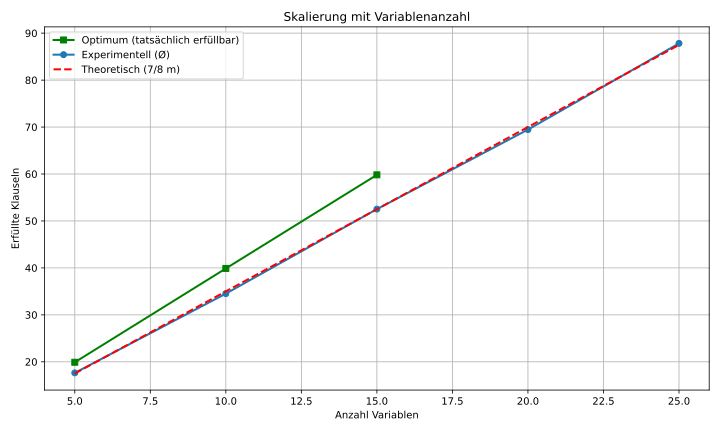
\includegraphics[width=0.95\textwidth]{experiment-results.pdf}
	\caption{Experimentelle Ergebnisse des 3-KNF Algorithmus mit Zufall}
	\label{fig:experiments}
\end{figure}
Auf der x-Achse ist die Anzahl der Variablen und auf der y-Achse die Anzahl erfüllter Klauseln aufgetragen. In grün eingezeichnet ist die Anzahl der erfüllbaren Klauseln. In blau eingezeichnet ist die Anzahl der erfüllten Klauseln durch den 3-KNF Algorithmus mit Zufall und in rot eingezeichnet ist die erwartete Anzahl erfüllter Klauseln durch den 3-KNF Algorithmus mit Zufall.

Beobachtbar ist, dass die Anzahl der erfüllten Klauseln durch den 3-KNF Algorithmus mit Zufall der theoretischen erwarteten Anzahl erfüllter Klauseln entspricht. Bis zu einer Anzahl von 15 Variablen ist die Anzahl der erfüllten Klauseln durch den 3-KNF Algorithmus mit Zufall nicht so hoch wie die optimale, d.h. maximale, Anzahl erfüllbarer Klauseln.

\section{Wahrscheinlichkeitsverteilungen}

Wann immer die Lehre vom Zufall in der Mathematik so verlassen wird, dass sie in der Praxis nicht mehr anwendbar ist, verletzen wir das eigentliche Ziel der Mathematik in diesem wichtigen Thema. Beim Erwartungswert war dies schon der Fall, denn auf die Augenzahl 3,5 wird der Würfel nie zufällig fallen. Damit muss die Lehre vom Zufall in der Mathematik sehr vorsichtig entwickelt werden. Denn wenn man zum Beispiel den Versuch einen Würfel zu würfeln oft wiederholt, ist beobachtbar, dass die Abweichung vom Erwartungswert beachtlich ist.

Die bekannten Wahrscheinlichkeitsverteilungen der Mathematik sind für die unterschiedlichen Versuche mit diskreten Ereignissen mit großer Genauigkeit und Vorsicht anzuwenden. Wird ein Versuch in seiner Beschreibung auf eine Anwendung einer Wahrscheinlichkeitsverteilung überprüft, können kleinste Details in der Beschreibung des Versuchs entscheidend sein für die Wahl der Wahrscheinlichkeitsverteilungen. Wird ein Detail in der Beschreibung des Versuchs übersehen und eine andere Wahrscheinlichkeitsverteilung gewählt, kann dies in der Analyse für den Versuch zu einem anderen Ergebnis führen.

Im Folgenden werden die unterschiedlichen Wahrscheinlichkeitsverteilungen aufgeführt. Dabei sollen Gemeinsamkeiten auffallen und dahin führen, dass sie diese Verteilungen mit Genauigkeit und Vorsicht anzuwenden sind.

\subsection{Bernoulli-Verteilung}

Die Bernoulli-Verteilung beschreibt Versuche, bei denen es nur zwei mögliche Ereignisse gibt. Ein Ereignis wird als Erfolg bezeichnet und das andere als Misserfolg. Zum Beispiel kann beim Wurf einer Münze das Ereignis Kopf als Erfolg und das Ereignis Zahl als Misserfolg bezeichnet werden. Ebenso kann beim Würfeln eines Würfels das Ereignis, dass der Würfel auf die Augenzahl $6$ fällt, als Erfolg bezeichnet werden und alle anderen Ereignisse, dass der Würfel auf die Augenzahlen $1, 2, 3, 4$ oder $5$ fällt, als Misserfolg.

Für einen Versuch, der durch die Bernoulli-Verteilung beschrieben wird, wird eine Zufallsvariable $X$ definiert durch
\begin{align}
	X = 
	\begin{cases} 
		1, & \text{falls Erfolg eintritt} \\
		0, & \text{falls Misserfolg eintritt}
	\end{cases}
\end{align}
Die Wahrscheinlichkeit für den Erfolg wird mit $p$ bezeichnet, also $P(X = 1) = p$. Die Wahrscheinlichkeit für den Misserfolg ist dann $P(X = 0) = 1 - p$. Es ist wichtig zu beachten, dass die Summe aller Wahrscheinlichkeiten $p + (1-p) = 1$ ergibt. Damit ist der Versuch mathematisch vollständig beschrieben.

Der Erwartungswert einer bernoulli-verteilten Zufallsvariable $X$ berechnet sich wie folgt:
\begin{align}
	E[X] &= 1 \cdot P(X = 1) + 0 \cdot P(X = 0) \\
	&= 1 \cdot p + 0 \cdot (1-p) \\
	&= p.
\end{align}
Das bedeutet, bei einem Versuch, der durch die Bernoulli-Verteilung beschrieben wird, erwarten wir im Mittel den Wert $p$. Für den Münzwurf mit $p = \frac{1}{2}$ erwarten wir also den Wert $0{,}5$. Dieser Wert kann nicht eintreten, denn die Münze zeigt entweder Kopf oder Zahl. Der Erwartungswert beschreibt aber formal genau, was bei vielen Wiederholungen dieses Versuchs zu erwarten ist.

\begin{beispiel}
	Ein Basketballspieler trifft den Korb mit einer Wahrscheinlichkeit von $p = 0{,}7$. Bei einem einzelnen Wurf wird der Erfolg (Treffer) mit der Zufallsvariable $X$ beschrieben, die bernoulli-verteilt ist mit Parameter $p = 0{,}7$. Der erwartete Wert ist $E[X] = 0{,}7$.
\end{beispiel}

Die Bernoulli-Verteilung ist die einfachste aller Wahrscheinlichkeitsverteilungen. Sie ist die Grundlage für viele weitere Verteilungen. Wird ein Versuch, der durch die Bernoulli-Verteilung beschrieben wird, mehrfach unabhängig wiederholt, ergeben sich andere Wahrscheinlichkeitsverteilungen, die auf der Bernoulli-Verteilung aufbauen.

\subsection{Geometrische Verteilung}

Die geometrische Verteilung beschreibt Versuche, bei denen ein Bernoulli-Versuch so oft wiederholt wird, bis zum ersten Mal ein Erfolg eintritt. Es stellt sich die Frage: Wie viele Versuche sind nötig, bis der erste Erfolg eintritt? Beim Würfeln eines Würfels kann man fragen: Wie oft muss der Würfel geworfen werden, bis zum ersten Mal die Augenzahl $6$ fällt? Bei diesem Versuch wird der Würfel so lange geworfen, bis die Augenzahl $6$ das erste Mal erscheint.

Für einen Versuch, der durch die geometrische Verteilung beschrieben wird, wird eine Zufallsvariable $X$ definiert durch
\begin{align}
	X = \{\text{Anzahl der Versuche bis zum ersten Erfolg}\}.
\end{align}
Die Wahrscheinlichkeit, dass der erste Erfolg genau beim $k$-ten Versuch eintritt, berechnet sich wie folgt. Es müssen zunächst $k-1$ Misserfolge eintreten, jeder mit Wahrscheinlichkeit $1-p$, und dann muss beim $k$-ten Versuch ein Erfolg mit Wahrscheinlichkeit $p$ eintreten. Damit ergibt sich:
\begin{align}
	P(X = k) = (1-p)^{k-1} \cdot p, \quad k = 1, 2, 3, \ldots
\end{align}
Es ist wichtig zu überprüfen, dass die Summe aller Wahrscheinlichkeiten $1$ ergibt. Dies ist tatsächlich der Fall, denn es gilt:
\begin{align}
	\sum_{k=1}^{\infty} P(X = k) = \sum_{k=1}^{\infty} (1-p)^{k-1} \cdot p = p \cdot \frac{1}{1-(1-p)} = p \cdot \frac{1}{p} = 1.
\end{align}
Damit ist der Versuch mathematisch vollständig beschrieben.

Der Erwartungswert einer geometrisch verteilten Zufallsvariable $X$ beträgt:
\begin{align}
	E[X] = \frac{1}{p}.
\end{align}
Das bedeutet, im Erwartungswert benötigen wir $\frac{1}{p}$ Versuche bis zum ersten Erfolg. Für das Würfeln einer $6$ mit einem Würfel ist $p = \frac{1}{6}$. Damit erwarten wir $E[X] = \frac{1}{1/6} = 6$ Würfe bis zum ersten Mal die Augenzahl $6$ fällt. Dies ist ein intuitives Ergebnis. Wird der Versuch in der Praxis durchgeführt, kann es sein, dass die $6$ bereits beim ersten Wurf fällt. Es kann aber auch sein, dass die $6$ erst nach 20 Würfen das erste Mal fällt. Der Erwartungswert beschreibt das, was im Mittel über viele Wiederholungen dieses gesamten Versuchs zu erwarten ist.

\begin{beispiel}
	Ein Unternehmen ruft potenzielle Kunden an. Jeder Kunde kauft mit Wahrscheinlichkeit $p = 0{,}2$ das Produkt. Die Anzahl der Anrufe bis zum ersten Verkauf ist geometrisch verteilt mit Parameter $p = 0{,}2$. Im Erwartungswert sind $E[X] = \frac{1}{0{,}2} = 5$ Anrufe nötig bis zum ersten Verkauf.
\end{beispiel}

Die geometrische Verteilung zeigt, wie vorsichtig der Erwartungswert interpretiert werden muss. In der Praxis kann die tatsächliche Anzahl der benötigten Versuche erheblich vom Erwartungswert abweichen. Dies ist bei allen Wahrscheinlichkeitsverteilungen zu beachten.

\subsection{Gaußsche Verteilung}

Die Gaußsche Verteilung, auch Normalverteilung genannt, beschreibt kontinuierliche Ereignisse. Bis jetzt wurden nur diskrete Ereignisse betrachtet. Bei kontinuierlichen Ereignissen kann die Zufallsvariable jeden beliebigen Wert aus einem Intervall annehmen, zum Beispiel alle reellen Zahlen. Die Gaußsche Verteilung ist die wichtigste Verteilung für kontinuierliche Ereignisse in der Praxis.

Ein Beispiel für einen Versuch mit kontinuierlichen Ereignissen ist die Messung der Körpergröße von Menschen. Die Körpergröße kann jeden Wert aus einem bestimmten Intervall annehmen, zum Beispiel zwischen $150$ cm und $210$ cm. Die Körpergröße ist damit keine diskrete Größe wie die Augenzahl beim Würfeln, sondern eine kontinuierliche Größe.

Für einen Versuch, der durch die Gaußsche Verteilung beschrieben wird, wird eine Zufallsvariable $X$ definiert, die Werte aus den reellen Zahlen annehmen kann. Die Gaußsche Verteilung wird durch zwei Parameter beschrieben: den Erwartungswert $\mu$ und die Varianz $\sigma^2$. Der Erwartungswert $\mu$ gibt an, um welchen Wert herum die Zufallsvariable streut. Die Varianz $\sigma^2$ gibt an, wie stark die Zufallsvariable um den Erwartungswert streut. Die Standardabweichung $\sigma$ ist die Wurzel aus der Varianz. Die Wahrscheinlichkeitsdichte der Gaußschen Verteilung ist gegeben durch:
\begin{align}
	f(x) = \frac{1}{\sqrt{2\pi\sigma^2}} \cdot e^{-\frac{(x-\mu)^2}{2\sigma^2}}.
\end{align}
Abbildung \ref{fig:gauss-dist} zeigt die Gaußsche Verteilung.
\begin{figure}[htbp]
	\centering
	\includegraphics[width=0.85\textwidth]{gauss-dist.pdf}
	\caption{Gaußsche Verteilung}
	\label{fig:gauss-dist}
\end{figure}
Bei kontinuierlichen Verteilungen kann nicht mehr nach der Wahrscheinlichkeit für ein einzelnes Ereignis gefragt werden, denn diese ist immer $0$. Stattdessen wird nach der Wahrscheinlichkeit gefragt, dass die Zufallsvariable $X$ in einem bestimmten Intervall $[a, b]$ liegt. Diese Wahrscheinlichkeit berechnet sich durch das Integral:
\begin{align}
	P(a \le X \le b) = \int_a^b f(x) \, dx.
\end{align}
Es ist wichtig zu überprüfen, dass das Integral über alle möglichen Werte $1$ ergibt. Dies ist tatsächlich der Fall, denn es gilt:
\begin{align}
	\int_{-\infty}^{\infty} f(x) \, dx = 1.
\end{align}
Damit ist die Gaußsche Verteilung mathematisch vollständig beschrieben.

\begin{beispiel}
	Die Körpergröße von erwachsenen Männern in Deutschland ist annähernd normalverteilt mit Erwartungswert $\mu = 180$ cm und Standardabweichung $\sigma = 7$ cm. Die Wahrscheinlichkeit, dass ein zufällig ausgewählter Mann eine Körpergröße zwischen $173$ cm und $187$ cm hat, entspricht etwa $68\%$. Dies ist ein bekanntes Ergebnis der Gaußschen Verteilung: Etwa $68\%$ aller Werte liegen im Intervall $[\mu - \sigma, \mu + \sigma]$.
\end{beispiel}

Die Gaußsche Verteilung hat eine besondere Eigenschaft: Viele Größen in der Natur und in der Praxis sind annähernd normalverteilt. Dies liegt daran, dass die Gaußsche Verteilung oft entsteht, wenn viele unabhängige Zufallseinflüsse zusammenwirken. Dieser Zusammenhang wird durch den Zentralen Grenzwertsatz der Mathematik beschrieben.

Es ist aber große Vorsicht geboten bei der Anwendung der Gaußschen Verteilung. Nicht jede Größe ist normalverteilt. Wird eine Größe fälschlicherweise als normalverteilt angenommen, können die Ergebnisse der Analyse völlig falsch sein. Zum Beispiel sind Aktienkurse nicht normalverteilt, obwohl dies oft angenommen wird. Extreme Ereignisse, sogenannte Ausreißer, treten bei Aktienkursen viel häufiger auf als die Gaußsche Verteilung vorhersagt. Dies kann zu erheblichen Fehleinschätzungen führen.

Die Gaußsche Verteilung ist ein mächtiges Werkzeug, aber sie muss mit Genauigkeit und Vorsicht angewendet werden. Nur wenn die Voraussetzungen für ihre Anwendung erfüllt sind, liefert sie zuverlässige Ergebnisse.

\section{Zusammenfassung}

In diesem Dokument wurde die Lehre vom Zufall in der Mathematik entwickelt. Ausgangspunkt war das einfache Beispiel des Würfelns eines Würfels. An diesem Beispiel wurden die grundlegenden Begriffe eingeführt: der Versuch, die Ereignisse, die Menge aller Ereignisse $\Omega$, und die Wahrscheinlichkeit für den Zufall eines Ereignisses. Es wurde gezeigt, dass ein Versuch mathematisch vollständig beschrieben ist, wenn die Summe aller Wahrscheinlichkeiten der Zufälle aller Ereignisse insgesamt $1$ ergibt.

Für die Analyse von Versuchen wurde das Konzept der Zufallsvariable eingeführt. Eine Zufallsvariable beschreibt den Zufall für das Ereignis variabel für den konkreten Ausgang. Mit Hilfe der Zufallsvariable kann der Erwartungswert berechnet werden. Der Erwartungswert beschreibt formal am genauesten, welcher Ausgang bei einem Versuch zu erwarten ist. Es wurde aber auch gewarnt, dass der Erwartungswert in der Praxis nicht immer sinnvoll interpretierbar ist. Beim Würfeln eines Würfels ergibt sich ein Erwartungswert von $3{,}5$, eine Augenzahl, die es nicht gibt. Der Erwartungswert beschreibt das, was im Mittel über viele Wiederholungen des Versuchs zu erwarten ist.

Am Beispiel des 3-KNF Algorithmus wurde gezeigt, wie Zufall in der Informatik eingesetzt wird, um effiziente Algorithmen zu entwickeln. Der Algorithmus mit Zufall für 3-KNF erreicht eine Approximationsgüte von $\frac{7}{8}$. Das bedeutet, dass im Erwartungswert mindestens $87{,}5\%$ aller erfüllbaren Klauseln erfüllt werden. Die experimentellen Ergebnisse zeigen, dass die theoretische Analyse mit der Praxis übereinstimmt. Dies ist ein Beispiel dafür, dass die mathematische Beschreibung des Zufalls in der Praxis anwendbar ist und zu verlässlichen Ergebnissen führt.

Die Wahrscheinlichkeitsverteilungen sind zentrale Werkzeuge für die Analyse von Versuchen mit Zufall. Es wurden drei Verteilungen vorgestellt: die Bernoulli-Verteilung für Versuche mit zwei möglichen Ereignissen, die geometrische Verteilung für die Anzahl der Versuche bis zum ersten Erfolg, und die Gaußsche Verteilung für kontinuierliche Ereignisse. Jede dieser Verteilungen hat ihre spezifischen Anwendungsbereiche. Es wurde mehrfach betont, dass die Wahl der richtigen Verteilung entscheidend ist. Kleinste Details in der Beschreibung des Versuchs können darüber entscheiden, welche Verteilung anwendbar ist. Wird eine andere Verteilung gewählt, führt dies zu anderen Ergebnissen in der Analyse.

Die Lehre vom Zufall in der Mathematik muss mit Genauigkeit und Vorsicht entwickelt und angewendet werden. Wann immer die mathematische Beschreibung so weit von der Praxis entfernt ist, dass sie nicht mehr anwendbar ist, wird das eigentliche Ziel der Mathematik in diesem Thema verletzt. Die Mathematik soll helfen, den Zufall zu verstehen und in der Praxis verlässliche Entscheidungen zu treffen.

\subsection{Ausblick}

Die in diesem Dokument vorgestellten Konzepte bilden die Grundlage für weiterführende Themen in der Wahrscheinlichkeitstheorie und Statistik. Es gibt viele weitere Wahrscheinlichkeitsverteilungen, die für spezifische Anwendungen entwickelt wurden. Die Binomialverteilung beschreibt die Anzahl der Erfolge bei mehrfacher Wiederholung eines Bernoulli-Versuchs. Die Poisson-Verteilung beschreibt die Anzahl von Ereignissen, die in einem festen Zeitintervall eintreten. Die Exponentialverteilung beschreibt die Wartezeit bis zum nächsten Ereignis. Jede dieser Verteilungen hat ihre eigenen Eigenschaften und Anwendungsbereiche, die sorgfältig studiert werden müssen.

Der Zentrale Grenzwertsatz ist ein fundamentales Ergebnis der Wahrscheinlichkeitstheorie. Er besagt, dass die Summe vieler unabhängiger Zufallsvariablen annähernd normalverteilt ist, unabhängig davon, welche Verteilung die einzelnen Zufallsvariablen haben. Dies erklärt, warum die Gaußsche Verteilung in der Natur und in der Praxis so häufig auftritt. Der Zentrale Grenzwertsatz ist die theoretische Grundlage für viele statistische Verfahren.

In der Statistik werden die Konzepte der Wahrscheinlichkeitstheorie verwendet, um aus Beobachtungen Schlüsse zu ziehen. Wenn wir einen Würfel mehrmals werfen und die Ergebnisse beobachten, können wir mit statistischen Methoden überprüfen, ob der Würfel fair ist. Wenn wir die Körpergröße von Menschen messen, können wir mit statistischen Methoden Rückschlüsse auf die Parameter der Verteilung ziehen. Die Statistik verbindet die theoretische Wahrscheinlichkeitsrechnung mit der praktischen Datenanalyse.

Der Einsatz von Zufall in Algorithmen, wie beim 3-KNF Algorithmus gezeigt, ist ein aktives Forschungsgebiet in der Informatik. Randomisierte Algorithmen können oft effizienter sein als deterministische Algorithmen. Sie werden in vielen Bereichen eingesetzt, von der Kryptographie über die Optimierung bis hin zum maschinellen Lernen. Das Verständnis der wahrscheinlichkeitstheoretischen Grundlagen ist essentiell, um solche Algorithmen zu entwickeln und zu analysieren.

Die Lehre vom Zufall in der Mathematik ist ein hilfreiches und vielversprechendes Gebiet gerade für die Entwicklung von Algorithmen. Sie verbindet abstrakte mathematische Konzepte mit konkreten praktischen Anwendungen und kann dabei helfen, Probleme effizienter zu lösen.
	
\end{document}